\documentclass[12pt,a5paper]{book}

\usepackage{../phffullpagefigure}

\usepackage{pdfpages}

\usepackage{lipsum}


\begin{document}

\lipsum[1-3]

And see Fig.~\ref{fig:test-1}. Placed using default side/placement, with figcontents command
[FIGCONTENTS].

\begin{fullpagefigure}
  \figcontents{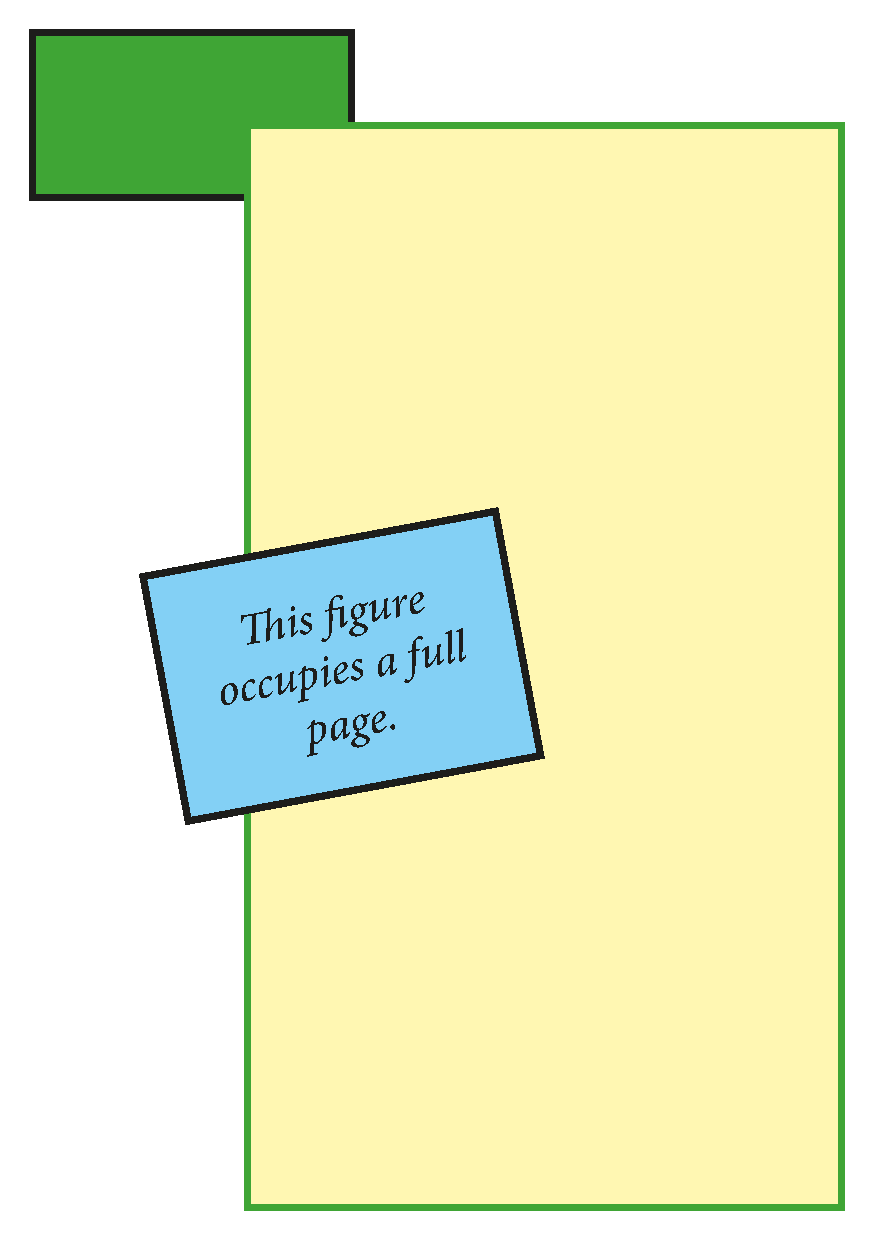
\includepdf{exampleA5fig}}
  \caption{Caption here. This is some text. This is some text. This is some text. This is
    some text. This is some text. This is some text. This is some text. This is some
    text. This is some text. This is some text. This is some text. This is some text. This
    is some text. This is some text. }
  \label{fig:test-1}
\end{fullpagefigure}

\lipsum[5-8]

\cleardoublepage
\lipsum[1-3]

And see Fig.~\ref{fig:test-1}. Placed using default side, with [p] flag [[P],FIGPDF].

\begin{fullpagefigure}[p]
  \figpdf{exampleA5fig}
  \caption{Caption here. This is some text. This is some text. This is some text. This is
    some text. This is some text. This is some text. This is some text. This is some
    text. This is some text. This is some text. This is some text. This is some text. This
    is some text. This is some text. }
  \label{fig:test-1}
\end{fullpagefigure}

\lipsum[5-7]

\cleardoublepage
\lipsum[1-3]

And see Fig.~\ref{fig:test-1}. Placed using default side, with [t] placement [FIGPLACEMENT,FIGPDF].

\begin{fullpagefigure}
  \figpdf{exampleA5fig}
  \figplacement{t}
  \caption{Caption here. This is some text. This is some text. This is some text. This is
    some text. This is some text. This is some text. This is some text. This is some
    text. This is some text. This is some text. This is some text. This is some text. This
    is some text. This is some text. }
  \label{fig:test-1}
\end{fullpagefigure}

\lipsum[5-7]

\cleardoublepage
\lipsum[1-3]

And see Fig.~\ref{fig:test-1}. Placed on an even side page [EVEN,FIGPDF].

\begin{fullpagefigure}
  \figpageside{even}
  \figpdf{exampleA5fig}
  \caption{Caption here. This is some text. This is some text. This is some text. This is
    some text. This is some text. This is some text. This is some text. This is some
    text. This is some text. This is some text. This is some text. This is some text. This
    is some text. This is some text. }
  \label{fig:test-1}
\end{fullpagefigure}

\lipsum[5-7]


\cleardoublepage
\lipsum[1-3]

And see Fig.~\ref{fig:test-1}, which is placed on an odd side page. [ODD,FIGPDF]

\begin{fullpagefigure}
  \figpageside{odd}
  \figpdf{exampleA5fig}
  \caption{Caption here. This is some text. This is some text. This is some text. This is
    some text. This is some text. This is some text. This is some text. This is some
    text. This is some text. This is some text. This is some text. This is some text. This
    is some text. This is some text. }
  \label{fig:test-1}
\end{fullpagefigure}

some small paragraph.

\FlushAllFullPageFigures

A new paragraph, after the flush command.

\lipsum[5-7]


\cleardoublepage
\lipsum[1-3]

And see Fig.~\ref{fig:test-1}. Placed on an even side page [EVEN,FIGPDF].

\begin{fullpagefigure}
  \figpageside{even}
  \figpdf{exampleA5fig}
  \caption{Caption here. This is some text. This is some text. This is some text. This is
    some text. This is some text. This is some text. This is some text. This is some
    text. This is some text. This is some text. This is some text. This is some text. This
    is some text. This is some text. }
  \label{fig:test-1}
\end{fullpagefigure}

\lipsum[5-7]



\end{document}
